
\documentclass[a4paper,12pt,twoside]{memoir}

%inkluderte pakker

\usepackage[utf8]{inputenc}
\usepackage{hyperref}
\usepackage{paralist}
\usepackage{graphicx}
\usepackage{cite}
\usepackage[table]{xcolor}
%\usepackage{biblatex}Tied to make chapref didnt work


%slutt på pakkene


%Styler kapittelet
\chapterstyle{veelo}

%bibtex resources
%\addbibresource{./kilder_bibtex/bib_iu_sjek.bib}
%\addbibresource{./kilder_bibtex/bib_iu_sykd.bib}
%\addbibresource{./kilder_bibtex/bib_iu_pro.bib}chapref

%Seksjoner, subseksjoner og paragrafutseende begynner her:
\setsecheadstyle{\bfseries\sffamily}   
\setsubsecheadstyle{\bfseries\sffamily}
\setsubsubsecheadstyle{\bfseries\sffamily}
\setparaheadstyle{\normalfont\footnotesize\bfseries\itshape\sffamily}
\renewcommand{\cftchapterfont}{\sffamily}   
\renewcommand{\cftsectionfont}{\sffamily}

%og slutter her


%Dette styrer fontene på overskriftene, starter her
\makeatletter
\g@addto@macro\chapnamefont{\sffamily} 
\g@addto@macro\chapnumfont{\sffamily}  
\g@addto@macro\chaptitlefont{\sffamily}
\makeatother
%slutter her

\setsecnumdepth{subsection}%numerer ned til dette nivået
\settocdepth{subsection}


\begin{document}
\sffamily

%%Her begynner oversettelsen til norsk
			\renewcommand{\partname}{Del}
			\renewcommand{\chaptername}{Kapittel}
            \renewcommand{\contentsname}{Innhold}
            \renewcommand\listfigurename{Illustrasjoner}
            \renewcommand\tablename{Tabell}
			\renewcommand\listtablename{Tabeller}
            \renewcommand{\figurename}{Illustrasjon}
			\renewcommand{\bibname}{Kilder:}
%%Her slutter den

\frontmatter
	%Grafisk Forside
	
	\newcommand\nbvspace[1][3]{\vspace*{\stretch{#1}}}
	% allow some slack to avoid under/overfull boxes
	\newcommand\nbstretchyspace{\spaceskip0.5em plus 0.25em minus 0.25em}
	% To improve spacing on titlepages
	\newcommand{\nbtitlestretch}{\spaceskip0.6em}
	\pagestyle{empty}
	\begin{center}
	\bfseries
	\nbvspace[1]
	\Huge
	{\nbtitlestretch\huge
	Kompendium\\ Legevakta i Drammen IKS}

	\nbvspace[1]
	\normalsize

	Internundervisning for sykepleierene\\
	med pasienteksempler\\
	\nbvspace[1]
	\small av\\
	\Large Pål Ager- Wick\\[0.5em]
	\footnotesize Fagsjef\\

	\nbvspace[2]

	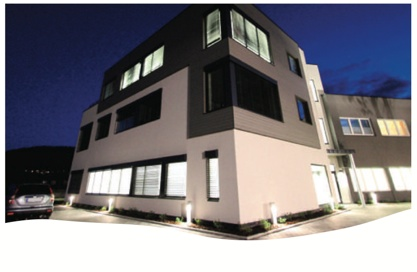
\includegraphics[width=6in]{./kap_pref/forsidelvdr.jpg} %placeholder for ete bilde på forsiden
	\nbvspace[3]
	\normalsize

	Drammen\\
	\large
	01.11.2013\\
	\nbvspace[1]
	\end{center}

%Slutt grafisk forside
			\chapter{Forord}%!!!
				Dette er et kompendium for internundervisningen ved Drammen IK legevakt. Det vil bli løpende oppdatert og være en del av fagutviklingen for sykepleierene, temaene vil bli lagt til etterhvert. Forløpig vil undervisningen være planlagt til mai -14.
				\\[0.7in]



				DRAMMEN 26.10.2013\\[0.4in]

				\emph{Pål CJ Ager-Wick}

	\newpage
	\tableofcontents
	%\begin{framed}
	%\end{framed} brukes for å ramme inn. Innhold er mellom.
\mainmatter
	\part{Sykdommer i praksis}	
		%\begin{refsection}
			\chapter{Hvordan jobbe systematisk}
		\section{Hva må du huske fra dette foredraget}
			\begin{itemize}
				\item Du må gjøre de du jobber sammen med så flinke som mulig, du spiller på et lag.\\
				\item Vi kommer alle til å gjøre feil. Meld fra sånn at de du jobber med slipper å gjenta feilen.\\
				\item Legen er også en del av teamet.\\
				\item Sjekklister hjelper oss å huske de kjedelige tingene vi vanligvis glemmer.\\
				\item Vær kritisk til all informasjon du får, du kan forvente at man skal kunne forklare hvorfor.\\
				\item Alle har ansvar for å lære, men det største ansvaret har du.\\
			\end{itemize}
		\section{Å lage verktøy for å ikke være redd}
			\paragraph{Hvorfor blir vi engstelige?\\}
				Det er utfordrende å jobbe i fremste rekke. Risikoen kan være høy. Men hva skjer dersom noe går galt. Mange av mottakerne av hjemmetjenester er eldre eller har flere sykdommer. Det kan være vanskelig kjenne igjen symptomer på alvorlige sykdommer, men også hva de forskjellige trenger. Noen ganger skjer ting som gjør helsepersonellet usikre eller redde.
			\paragraph{Glemsk?\\}
				Det er alltid mye nytt om behandling av kjente sykdommer. Det kan være veldig mye å sette seg inn i. Den menneskelige hjerne kan huske 7-9 ting på en gang. Det kan være utfordrende huske på alt sammen. Men samtidig kan vi som helsepersonell mye om sykdommer. Huskelister kan være en måte å redusere komplikasjoner på\cite{FA-gawande}.
		\section{Lær av feil}
			\paragraph{Endel av hverdagen vår\\}
				Å være helsepersonell vil gjøre at man må håndtere feil. Det er ingen som ønsker å gjøre feil, men det hender likevel alle. Når det skjer er det desto viktigere å lære av dem.
			\paragraph{I system\\}
				For å unngå å gjennta feil eller avdekke dem på systemnivå, må vi ha et system for å fange dem opp. Avviksmeldinger kan være kjedelig ekstraarbeid som kommer på toppen av alt i en travel hverdag. Likevel er det bare slik man kan lære.
		\section{Hvordan finne god informasjon}
			\paragraph{Jeg lurer på...\\}
				Hvor slår du opp hvis du lurer på noe. Det er ikke sikkert at alle internettkilder er like pålitelige. Hvem svarer på alle spørmålene som dukker opp i løpet av en travel arbeiddag. Det er veldig viktig å ha system på dette for å sørge for at all informasjonen vi bruker er kvalitetssikret. 
			\paragraph{Hvem bestemmer hvordan pasienter skal behandles?\\}
				Det finnes mange veiledere fra helsedirektoratet som gir retningslinjer. Andre ressurser er \href{http://www.helsebiblioteket.no/}{helsebiblioteket.no}. Det viktigste er at alle i tjenesten engasjeres i å utvikle faget, og at man får tid til det. 
		%\section{Sjekklister fra bakken og opp?}
		%\section{Systemer er kjedelig} Beholde?
		%\section{Noen praktiske prinsipper} %Systematisk arbeid kapittelet
			\chapter{Hjertesykdommer}
			\chapterprecishere{40 \% av alle nordmenn dør av hjerte- karsykdommer\raggedleft--- \textup{Statistisk sentralbyrå, Dødsårsaksregisteret\\[0.5in]}}
		
		\section{Perlene...}
			\begin{itemize}
				\item Hjertesvikt er ikke en egen sykdom men en beskrivelse av nedsatt hjertefunksjon.\\
				\item NYHA beskriver hvor alvorlig hjertesvikten er og er basert på hvordan pasientene fungerer i hverdagen.\\
				\item Hjertesvikt har høy dødelighet.\\
				\item De eldste, kvinner og pasienter med diabetes har ofte helt utypiske symptomer på hjerteinfarkt.\\
				\item Digitalis har lang halveringstid i kroppen.\\
				\item Diare og slapphet er vanligste symptomer ved digitalisoverdose.\\
				\item Digitalis brukes i behandling av atrieflimmer for å stabiliserer hjerterytmen.\\
			\end{itemize}

		\section{Noen sykdommer av mange}	
			Her er noen få av alle hjertesykdommene forklart. Dette er ment å være et tillegg til forelesningen slik at man ikke må notere så mye. Dette er ikke en fullstendig oversikt over hjertesykdommene. Det er også forsøkt å forklare på et så enkelt som mulig nivå slik at hjertespesialister eller andre vil føle at det er litt enkelt. Dette materialet er ikke laget for dem.\\
		\section{Anatomi}
					\begin{figure}[ht]
                      \centering
                      	\frame{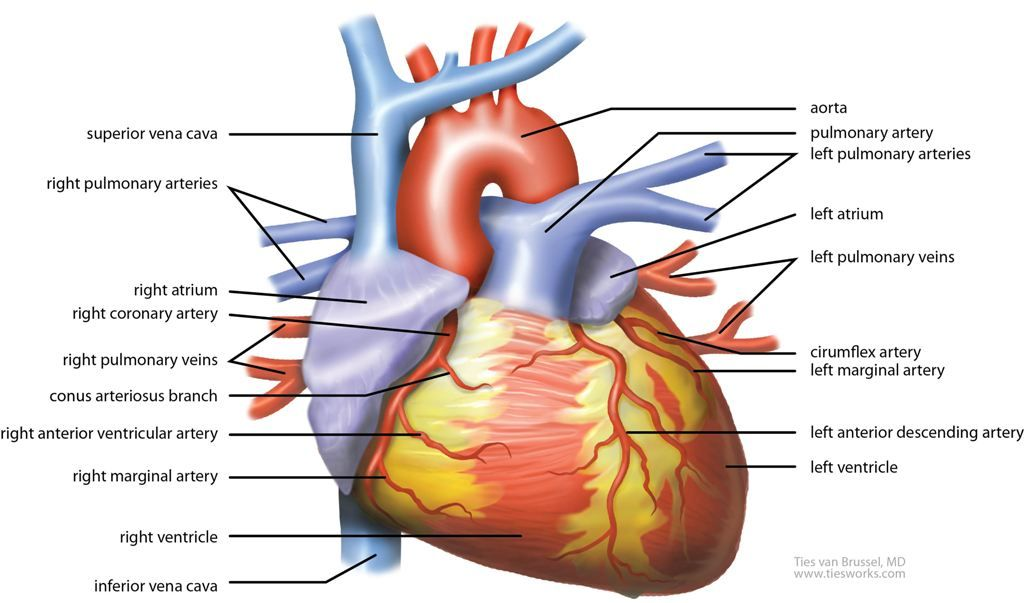
\includegraphics[width=5in]{./kap_syk/bilder/hjertebedre.jpg}}
                      \caption{Et hjerte}
                      %{Her ser vi et hjerte som er fiksert i formalin.}%\textit{tjenestetilbudene}.]
                    \end{figure}    


				%!!! Her må et bilde inn
			\paragraph{Effektiv jobbing\\}
				Når hjertet pumper med vanlig frekvens er det veldig effektivt. Da sørger det for jevn transport av blodet på en mest mulig energieffektiv måte. Når hjerteslagene blir veldig raske blir hjertet mindre effektivt\cite{FA-saladin}. Man kan kalle det en funksjonell hjertesvikt. Det betyr at hjertet er friskt, men jobber på- eller over grensen for at blodet skal strømme fritt.
				%legg inn video an ultralyd ecco cor!!!
		\section{Fysiologi}	
			\paragraph{Hva menes med hjerte- og karsykdommer?\\}\label{sec:athero}
				Som alle organer i kroppen har hjertet sine egne blodårer. De er ekstra utsatt for åreforkalking, eller atherosklerose som det heter på latin. Atherosklerose er kalkinnlagring i blodåreveggen som gjør den stiv og samtidig klumpete på innsiden. Dette hindrer blodgjennomstrømningen. Mengden med kalk i blodårene er varierende gjennom livet, men fet mat, høyt blodtrykk og sigaretter gjør at mer kalk lagres. 
		\section{Patologi}	
			\paragraph{Skader oppstår\\}
				Noen steder blir blodpassasjen dårlig og det kan dannes skader fordi vevet ikke får nok oksygen. Hjertet er en muskel med innebygget nervesystem og noen ganger blir det små skader som gror til arr i forkammeret. Dette kan skape atrieflimmer\cite{!!!}. Hvis blodårene tetter seg rundt hjertekammeret får man ofte anginasmerter, og dersom blodåren blir helt tett er det et infarkt.
		\section{Klinikk}
			\subsection{Hjerteinfarkt}	
				\paragraph{Symptomer\\}
					Trykkende smerte i brystet, utstråling til venstre arm eller underkjeve. Blek og kaldsvett, klam og tungpusten. Dette er noen klassiske symptomer ved hjerteinfarkt. Vi må passe oss fordi, eldre, pasienter med diabetes eller kvinner har ofte helt andre symptomer. 
				\paragraph{Førstehjelp\\}
					Ring ambulansen, vær hos pasienten. Gi oksygen og Dispiril hvis dere har. 
				\paragraph{Farlige momenter\\}
					De som dør av hjerteinfarkt får ofte akutt hjertflimmer. Dette er ikke atriflimmer, men kammerflimmer og er helt forskjellig. Hjertet slår med 300 slag i minuttet. Pasienten er bevisstløs og den eneste redningen er å bruke hjertestarter og å gjøre hjerte- lungeredning. Det viktigste for akutte hjerteinfarkt er rask behandling med utblokking og innsetting av stent. Noen pasienter egner seg ikke for dette, særlig de eldste og sykeste ville ikke overleve behandlingen og blir heller behandlet på sykehus uten utblokking. 
				\paragraph{Hva skjer etterpå?\\}
					Alle pasienter som har hatt hjerteinfarkt får nesten samme type medisiner:
					\begin{itemize}
						\item Metoprolol(SelZok \textregistered), gjør at hjertet for "hvile". Forebygger nye infarkt og hjerterytmeforstyrrelser. Senker blodtrykket, og gjør at makspulsen blir lavere ved fysiske anstrengelser. Noen menn blir impotente. Kalles også "Betablokker"\\
						\item Acetylsalisylsyre(Albyl-E\textregistered) \\
						\item ACE- hemmer(Renitec \textregistered) eller AT\textsubscript{2}-antagonister(Cozaar \textregistered, eller andre), senker blodtrykket.\\
						\item Statiner(Simvastatin, Atorvastatin(Lipitor\textregistered)), senker farlig kolesterol og stabiliserer crispy blodårer.\\
					\end{itemize}
				\paragraph{Tips for hverdagen\\}
					Hjertesyke pasienter bør man passe på brå endringer i tilstanden, dette gjelder forøvrig alle andre sykdomstilstander som blir beskrevet her. Hvis en pasient har kjent hjertesykdom og lav "blodprosent" kan den lave blodprosenten utløse infarkt.
			\subsection{Hjertesvikt}
				Er oftest en komplikasjon etter et hjerteinfarkt som ikke ble behandlet i tide. New York Heart Assosiation(NYHA) har klassifisert hjertesvikt etter hvordan pasientene fungere i hverdagen. 
					\begin{table}[ht]
						\caption{NYHA(New York heart assosiation) klassifisering av hjertesvikt}
						\centering
						\rowcolors{1}{cyan}{white}
						\begin{tabular}{|p{2cm}| p{11cm}|}
							\hline
							\textbf{KLASSE} & \textbf{Symptomer}\\[0.75pt]
							\hline
							1 (I) & Hjertesvikt uten kliniske symptomer\\
							\hline
							2 (II) & Hjertesviktsymptomer (dyspné, takykardi, tretthet) kun ved\newline større fysiske anstrengelser som rask gange i motbakke. \newline Pasienten kan gå 2–3 etasjer i trapp sammenhengende\\
							\hline
							3 (III) & Symptomer ved moderat fysisk anstrengelse som dagliglivets aktiviteter,\newline rolig gange på flat vei eller gange opp en etasje i trapp\\
							\hline
							4 (IV) & Symptomer i hvile eller ved minimal aktivitet som personlig stell \\
							\hline
						\end{tabular}
					\end{table}
				\paragraph{Symtomer\\}
					Tungpust og hovne bein. Slapphet og trettbarhet. Dårlig matlyst.
				\paragraph{Hva må helsepersonell passe på\\}
					Følg med på vekten. En hjertesviktpasient kan gå opp i vekt med flere kilo om dagen dersom medisinene slutter å fungere. 
				\paragraph{Hvor farlig er det\\}
					Jo høyere grad hjertesvikt jo dødligere er det. En alvorlig hjertesvikt er å sammenligne med kreftsykdommer med spredning. Ikke glem å rådføre med lindrende avdeling når det gjelder disse pasientene.
				\paragraph{Tips for hverdagen\\}
					Ikke glem å veie hjertesviktpasienter. Alle med hejrtesvikt bør føre drikkeskjema fordi for mye drikke kan forverre symptomene. 
			\subsection{Atrieflimmer}
				Noen ganger utvikler hjertet en feil i det elektriske systemet. Dette fører til atrieflimmer, som ofte kommer anfallsvis. Når blodet utsettes for ujevne hjerteslag kan det klumpe seg og føre til hjerneslag.
				\paragraph{Symptomer\\}
					Samme som hjertesvikt, men kommer ganske akutt. Pulsen er ujevn og rask. 
				\paragraph{Hva må hjemmetjenesten være oppmerksomme på?\\}
					Å drikke lite gjør at pasientene kan få anfall. Hvis blodfortynningen ikke er tilstrekkelig, vil pasientene kunne få slag. Derfor er det viktig å følge med på INR. 
				\paragraph{Medisiner\\}
					Metoprolol begrenser hjerterytmen og forebygger anfall. Marevan forebygger hjerneslag. Noen nye behandlinger er under innføring for eksempel Rivaroxiban (Xarelto\textregistered), som også virker blodfortynnende. Noen pasienter får Digitalis(Digoxin \textregistered, Digitoxin \textregistered, som det står mer om i neste kapittel.
			\subsection{Digitalis}
				Digitalis er et naturprodukt som er veldig giftig. Det styrker hjertemuskelens evne til å slå og stabiliserer hjerterytmen.
				\paragraph{Litt om farmakologi\\}
					Terapeutisk bredde betyr at man har lite spillerom med dosen til et legemiddel. Det vil si at en liten økning i dosen kan være farlig eller dødelig. \\
					Halveringstid: Betegner hvor lenge et legemiddel bruker på reisen gjennom kroppen.\\
				\paragraph{Load and go...\\}
					Digitalis har smal terapeutisk bredde, og treg passasje gjennom kroppen. Det betyr at selv ved små økninger i dosen er det lett å bli forgiftet. Det tar også lang tid å få digitalis ut av systemet, ofte flere uker dersom man har hatt for høy dose lenge. Digitalis trenger også en loading dose ved oppstart. Det betyr at en høyere dose gis ofte de første dagene for å få effekt.
				\paragraph{Rare symptomer\\}
					Fordi digitalis er lett å overdosere skjer det nokså ofte, men oppdages også sent. Det er fordi symptomene er vanskelige å skille fra andre tilstander. Kvalme, diaré og forvirring er ikke uvanlig hos eldre, men akkurat disse tre er typisk for forgiftning med Digitalis.
				\paragraph{Praktisk råd:\\}
					Hvis en pasient bruker digitalis og får diaré bør lege kontaktes. Det kan skyldes forgiftning. Husk at diaré også kan føre til at Digitalis kan bli tatt opp annerledes i kroppen.
		\section{Pasienteksempler}
			\subsection{Pasient 1}
			\subsection{Pasient 2}



\newpage %hjertekapittelet
		\chapter{Nevrologiske sykdommer}
		\section{Hva du skal ta med deg videre:}
			\begin{itemize}
				\item Husk FAST -Fjes -Arm -Språk -Tid.\\
				\item Ta et blodsukker.\\
				\item Drypp er en av de største risikofaktorene for slag.\\
				\item Slagpasienter som sliter språklig er ikke dumme.\\
				\item Regelmessig puls?\\
			\end{itemize}
		\section{Kort om denne delen...}
			Hjernen er hoveddelen av sentralnervesystemet. Det er ikke meningen å snakke om hele nervesystemet, men denne delen omhandler slag, drypp og demens som er noen av de største utfordringene vi har i dag. Jeg kommer ikke til å bruke mye pass på parkinsons og andre sykdommer da dette ville blitt for omfattende for dette dagsseminaret.
		\section{Anatomi}
			\paragraph{Et komplekst bilde}
				\begin{figure}[ht]
                      \centering
                      	\frame{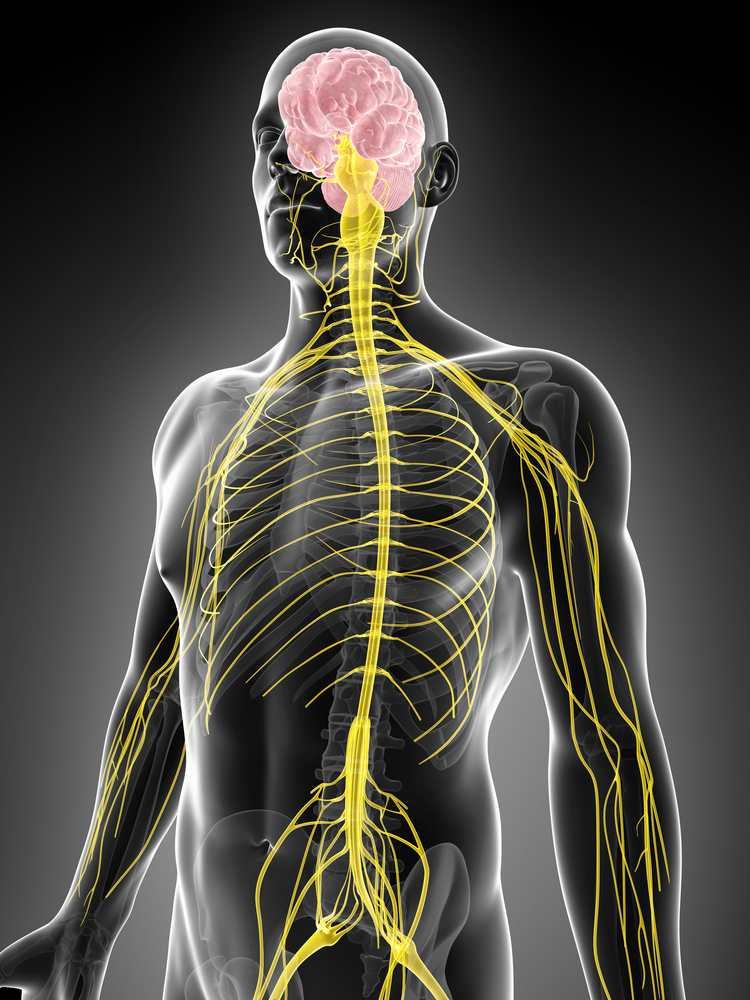
\includegraphics[width=3in]{./kap_syk/bilder/nevro1.jpg}}%!!! må byttes ut, copyright Greys anatomy
                      \caption{Oversiktsbilde over det sentrale nervesystem}
                      %{Her ser vi et bilde som illusterer lungene og den antomiske oppbygningen}%\textit{tjenestetilbudene}.]
                    \end{figure}
			\paragraph{Inndelingen\\}
				Hjernen er forbundet med ryggmargen i medulla oblongata, eller den forlengede ryggmargen på norsk. Selve ryggmargen går omlag 2/3 ned av hele lengden av ryggen. 
		\section{Fysiologi}
			\paragraph{Kompleks struktur\\}
				Hjernen er organisert i områder som jobber med hver sine oppgaver. For eksempel sitter personligheten foran, rett bak pannen. Alle nervecellene er koblet sammen som et stort nettverk som løser hver sine oppgaver, men også jobber på kryss og tvers. 
			\paragraph{Plastisitet\\}
				En viktig egenskap er kalt "Hjernens plastisitet". Det betyr at hjernen kan reparere og til dels få tilbake tapte funksjoner igjen. for eksempel kan en person som har hatt slag trene seg opp ved å bruke en annen del av hjernen enn den som ble skadet. 	
		\section{Patologi}
			\paragraph{Sykdommer i blodårene\\}
				Som beskrevet i \nameref{sec:athero} på side \pageref{sec:athero} %!!!
				er årsaken til slag og drypp en forkalking av blodårene og en plutselig tiltetting av disse\cite{FA-athero}. Det som følger er omtrent som ved hjerteinfarkt: en del av hjernen mister oksygentilførselen og nervene dør. Ettersom hvor den tette åren sitter blir symptomene lokalisert på kroppen.
				%Homonkulus bilde!!!
			\paragraph{Sykdommer i nervescellene\\}
				Demens forårsakes av at det lagres et protein som heter tau(egentlig den greske bokstaven T), og som ødelegger nervecellene det lagres inne i. Det finnes flere typer demens og behandlingen er forskjellig. Mest kjent er Alzheimers demens. I dag er demens en sykdom som ikke har god behandling. Det finnes noen medisiner som reduserer symptomer men det er oftest kortvarig. 
		\section{Klinikk}
			\subsection{Slag og drypp}
			\subsection{Demens}
				\subsubsection{Alzheimers}
				\subsubsection{Andre former for demens}
		\section{Pasienteksempler}
			\subsection{Pasient 3}
			\subsection{Pasient 4}


\newpage %nevrologikapittelet	
		\chapter{Lungesykdommer}
		%\chapterprecishere{Vuuuu, vuu vuu\par\raggedleft--- \textup{Molly}, En husky hund fra Drammen}
		\section{Dette har du lært}
			\begin{itemize}
				\item KOLS er underdiagnostisert i Norge.\\
				\item Det er tre spørsmål alle må kunne\cite{anthonisen}:\\
					\begin{itemize}
						\item Hoster du mer enn du pleier?\\
						\item Kommer det opp mer guffe enn vanlig?\\
						\item Er du mer tungpusten enn ellers?\\
					\end{itemize}
				\item KOLS pasienter skal vaksineres.\\
				\item Oksygen er et legemiddel.\\
				\item KOLS pasienter som blir innlagt på sykehus har høy dødelighet.\\
				\item Lavere terskel for antibiotika, for de med KOLS.\\
				\item Blodpropp i lungene er alvorlig og vanskelig å diagnostisere.\\
			\end{itemize}Her presenteres lungesykdommene vi snakker om i kurset. Målet er å lære om KOLS. Forskjellen på KOLS og astma. Lungebetennelse, blodpropp og andre tilstander i lungene beskrives også, men kort.
		\section{Anatomi}
			\paragraph{Stor overflate\\}
				\begin{figure}[ht]
                      \centering
                      	\frame{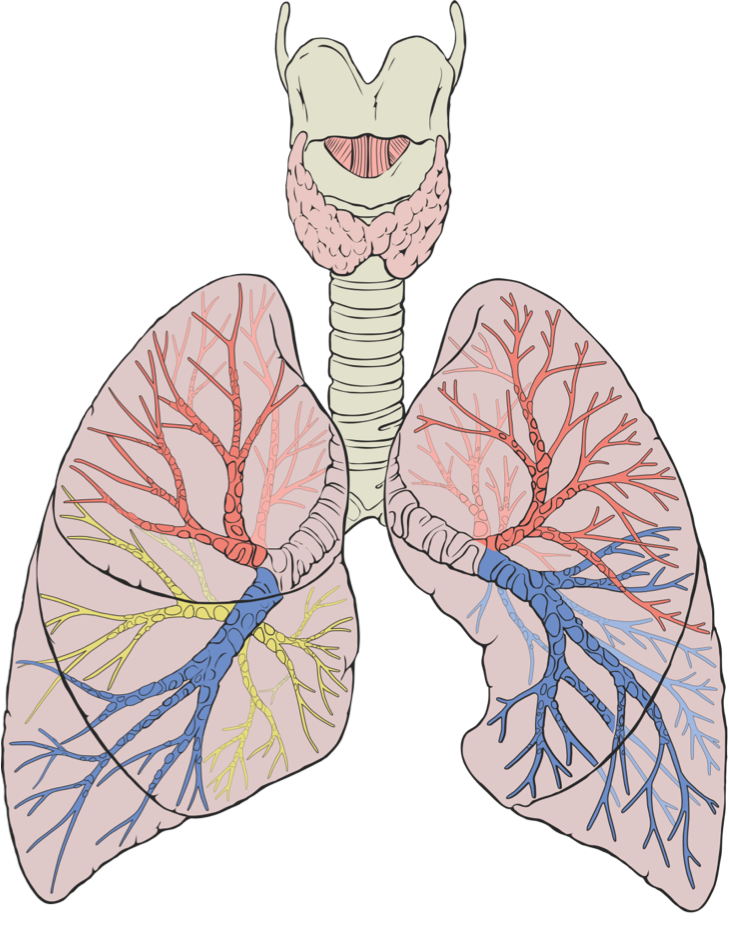
\includegraphics[width=4in]{./kap/bilder/lungeskjema.png}}%!!! må byttes ut, copyright Greys anatomy
                      \caption{Et lungebilde}
                      {Her ser vi et bilde som illusterer lungene og den antomiske oppbygningen}%\textit{tjenestetilbudene}.]
                    \end{figure}
            \paragraph{300 millioner\\}
            	En enorm overflate er nødvendig for effektiv utveksling av oksygen og carbondioksid. Lungene er delt i lapper. Gasutvekslingen finner sted i alveolene(som det finnes 300 millioner av). Lungene har samme overflate som en tennisbane.
		\section{Fysiologi}
				\paragraph{Syre- base\\}
					CO\textsubscript{2} påvirker sammen med bicarbonat syre- base i lungene. Det er en av grunnene til at det tas blodgass av KOLS pasienter. Det kan også bidra til at pasienter med lungesykdommer kan være ustabile.
				\paragraph{Litt om O\textsubscript{2}\\}
					Oksygen kommer inn i kroppen via lungene. Det er ingen andre veier inn. 
		\section{Patologi}
			\paragraph{Arrvev\\}
				Det oppstår arrvev og skader som ødelegger alveolene (emfysem) og obstruksjon av luftveiene hinder luftpassasje i de større luftveiene. Sammen gjør dette at overflaten blir mindre.
			\paragraph{Emfysem\\}
				Konsekvensen av arrvev i lungene kan være store deler av lungen som forsvinner og store hulrom med luft er alt som er igjen. 
					\begin{figure}[ht]
                      \centering
                      	\frame{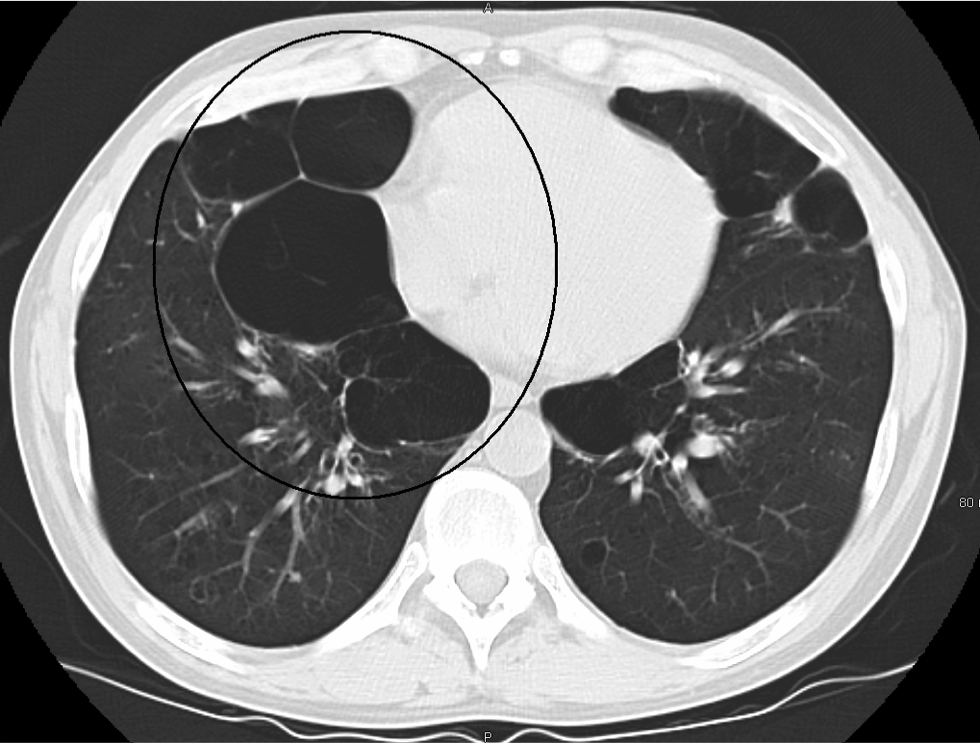
\includegraphics[width=5in]{./kap/bilder/emfysemct.png}}%!!! må byttes ut, copyright Greys anatomy
                      \caption{Et CT-bilde av en emfysemlunge}
                      {Her ser vi et CT-bilde av lunger med emfysem. Dette er ikke alltid mulig å se på vanlig røntgen. Det samme gjelder med ultralyd.}%\textit{tjenestetilbudene}.]
                    \end{figure}
            \paragraph{Andre problemer\\}
            	Mange andre tilstander påvirker lungefunksjonen. Dette er ikke en fullstendig liste men: pneumothoraks, pleuravæske, lungebetennelser, lungeødem, lungearterieemboli og mange flere. Ofte er sykdomstilstanden kjent, men det er viktig å huske på at for eksempel KOLS pasienter har hyppigere pneumothoraks enn den vanlige befolkningen. Lærepoenget er at vi skal huske på at vi må gjøre diagnostikk, selv på velkjente KOLS pasienter med forverringer. 
		\section{Klinikk}
			\subsection{KOLS}
				\paragraph{Største pasientproblemer\\}
					Tungpust er det største hinderet i hverdagen. For mange er belastningen med røykeslutt også en vanskelig byrde med sosiale konsekvenser. 
				\paragraph{Mange viktige målinger\\}
					Spirometri gir diagnosen KOLS. Klassifiseringen er GOLD, stadium I-IV, hvor IV er mest alvorlig.
						\begin{figure}[ht]
                      \centering
                      	\frame{
\includegraphics[width=6in]{./kap/bilder/goldnorsk.png}}%!!! må byttes ut, copyright GOLD
                      \caption{GOLD klassifiksjonen}
                      %{Her ser vi et bilde som illusterer lungene og den antomiske oppbygningen}%\textit{tjenestetilbudene}.]
                    \end{figure}
			\subsection{Pneumoni}
				Infeksjoner i lungene er veldig vanlig. Vanligvis kan dette behandles med penicillin, men ikke hos KOLS pasienter. Symptomer er: Feber, slapphet og produktiv hoste. Det er ikke uvanlig med septiske forløp hos eldre. 
			\subsection{Lungeemboli}
				Blodpropper fra beina blir fanget i lungene dersom de løsner. Pasienter kan ha forkjellige symptomer, som tungpust, pusteavhengige smerter, smerter i brystet eller andre diffuse plager. Problem: Alle symptomene kan passe til andre sykdommer også.
		\section{Pasienteksempler}
			\subsection{Pasient 5}
			\subsection{Pasient 6}	%lungekapittelet
		\chapter{Urinveier}%urinveiene
		\section{Gullkornene:}
			\begin{itemize}
				\item Vanligere med urinveisinfeksjon i høyere alder.\\
				\item En vanlig årsak til delir(se side \pageref{delir}).\\
				\item Bakterier i urinen til gamle damer behøver ikke være farlig.\\
				\item Lukt og farge kan lure oss.\\
			\end{itemize}
		\section{Anatomi}
					\begin{figure}[ht]
                      \centering
                      	\frame{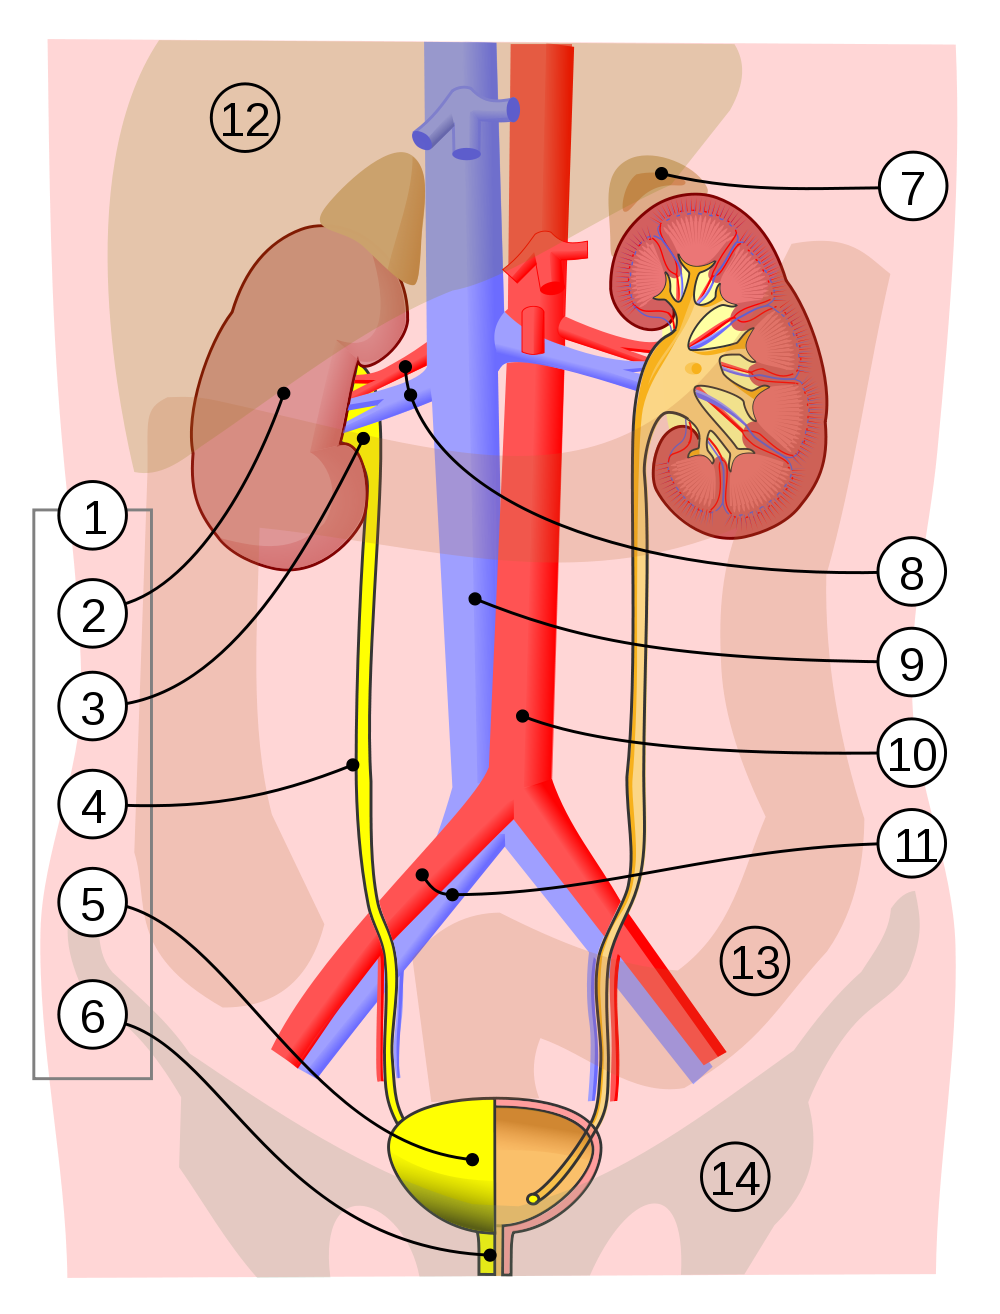
\includegraphics[width=5in]{./kap_syk/bilder/urinveier.png}}%!!! må byttes ut, copyright Greys anatomy
                      \caption{\emph{1.} Urinveiene ,\emph{2.} Nyre, \emph{3.} Nyrebekkenet, \emph{4.} Urether, \emph{5.} Blæra, \emph{6.} Urethra, \emph{7.} Binyre, \emph{8.} Nyrearterie og -vene, \emph{9.} Vena cava inferior, \emph{10.} Bukaorta, \emph{11.} Arteria og Vena Iliaca, \emph{12.} Lever, \emph{13.} Tykktarmen, \emph{14.} Bekkenet}
                    \end{figure}
			\paragraph{Feilkonstruksjon?\\}
				Kvinner har et kort urinrør som gjør det svært lett å få urinveisinfeksjoner. At eldre damer har bakterier i urinen uten symptomer er forholdsvis vanlig og ikke farlig\cite{uti-old}
			\paragraph{Den svake strålen\\}
				Menn har også hyppigere infeksjoner med alderen. Det er ofte prostaten, plager etter operasjon og kateterbruk som gjør dette. 
		\section{Fysiologi}
			Bakteriene vandrer nedenfra og opp. Urin er steril hos friske. Eldre med bakterier uten symptomer trenger vanligvis ikke behandling. 
		\section{Patologi}
			\paragraph{Flere nivåer\\}
				Bakteriene irriterer lokalt og skaper smerter når man er på do. Noen får generell slapphet av den pågående reaksjonen. Hvis bakteriene kommer opp til nyrene kalles det pyelonefritt, eller nyrebekkenbetennelse. Kommer de enda høyere kalles det urosepsis og er kjennetegnet av at bakteriene sprer seg i hele kroppen via blodet. 
		\section{Klinikk}
			\subsection{UVI}
				Veldig vanlig og trenger ikke behandling dersom fravær av symptomer. Pasienten bør følges tett dersom bakterier påvises, for deretter å kunne slippe opp litt. Man i disse pasientene huske på at urinveiene an være årsak ved sykdom. Ta urinprøver regelmessig, men det behøver ikke føre til behandling.
		\section{Pasienteksempler}
			\subsection{Pasient 7}
			\subsection{Pasient 8}%Nyrekapittelet
		\chapter{Delir}\label{delir}%Delir
		\section{Viktigeste momenter fra foredraget}
			\begin{itemize}
				\item Rammer nesten alltid de over 65 år.\\
				\item Delir er en brå forandring i det kognitive.\\
				\item Et symptom og ikke en sykdom.\\
				\item Har alltid en underliggende forverring eller nyoppstått sykdom, medisinbruk eller annen toksisk tilstand som årsak.\\
				\item Man behandler den utløsende årsaken. Haldol og andre medisiner er kun støttebehandling.\\
				\item Med urinprøve, et stetoskop og god sykehistorie kan man finne ut mye.\\
				\item Er ikke det samme som demens, men demente kan få det.\\
			\end{itemize}
		\section{Anatomi}
			Delir rammer hjernen og akkurat hva og hvordan den mentale forandringen foregår er ikke beskrevet i detalj\cite{rev_compre}\cite{pers_delir}.
		\section{Fysiologi}
			På grunn av det som er skrevet over er det vanskelig å gi en enkel forklaring på akkurat hva som fører til delir på cellenivå.
		\section{Patologi}
			Siden delir er symptom er det mangfoldige sykdommer som kan ligge bak. Her følger en kort oversikt\cite{legevakthandboka}.
				\paragraph{Oversikt over noen av tilstandene som går forut for delir\\}
					\begin{itemize}	
						\item Infeksjoner. Urinveisinfeksjon, pneumoni og sepsis, sjeldnere meningitt eller encefalitt.\\
						\item Medikamenter. Blant annet medikamenter med antikolinerg virkning, antiparkinsonmidler, opiater, sedativer, litium, digitoksin og blodtrykkssenkende midler.\\
						\item Metabolsk årsak. Blodsukkerendring. Tyreoideasykdom. Elektrolyttforstyrrelse, særlig hypo- og hypernatremi og hyperkalsemi. \\
						\item Syre- og baseforstyrrelse. Uremi (obs: nyresvikt, urinretensjon).\\
						\item Alkohol- eller rusmiddelseponering.\\
						\item Hypoksi, av ulike grunner, for eksempel hjertesvikt eller akutt redusert lungefunksjon.\\
						\item Kardiovaskulær årsak. Hjerteinfarkt, TIA, hjerneslag.\\
						\item Hodeskade. Obs — subduralt hematom.\\
						\item Frakturer. Obs — innkilt lårhalsbrudd hos demente.\\
						\item Epilepsi. Etter anfall.\\
						\item Underernæring. B-vitaminmangel.\\
						\item Hypo- og hypertermi.\\
					\end{itemize}

		\section{Klinikk}
			\paragraph{Mange symptomer}
				Utvikles vanligvis i løpet av timer til døgn. Oppmerksomhetssvikt, redusert hukommelse, desorientering. Gjerne døgnvariasjon i grad av forvirring. Uro og fikling (vandrer rundt, drar ut katetre eller venekanyler) eller tilbaketrukkethet. Noen hallusinerer. MMS skal ikke gjennomføres, fordi det gir ingen tilleggsinformasjon.
		\section{Pasienteksempler}
			\subsection{Pasient 9}
			\subsection{Pasient 10}%delirkapittelet
			\chapter{Diabetes i alderdommen}%diabetes og hypoglykemi
		\section{Punkter å ha med seg:}
			\begin{itemize}
				\item Diabetes hos eldre er resultat av for mye sukker i mange år.\\
				\item Hypoglykemi er den eneste metaboliske sykdommen som kan nevrologiske symptomer på bare en side.\\
				\item Proteiner ødelegger alt!\\
				\item Ikke glem at alle skal følges opp med øynene hvert år.\\
				\item Hvis pasienten har 5 mg/dl i blodsukker om kvelden og skal ha 15 IE Lantus\textregistered. så virker ikke Lantus før om morgenen etter.\\
			\end{itemize}
		\section{Anatomi og fysiologi}
			Sukker tas opp i tarmen, og ender i blodbanen. Insulin lages i bukspyttkjertelen(=pankreas), og styrer cellenes evne til å ta opp sukker ved å koble seg til cellene(viktig begrep: insulinreseptor) som en liten minnepinne med mye informasjon. Når cellene påvirkes av insulin skjer det masse, men sukkeret i blodbanen reduseres.
		\section{Patologi}
			\paragraph{Insulinresistent\\}
				Til slutt blir cellene lei av alt insulinet og reagerer med å ikke være mottakelige lenger. De er utslitte av all lagringen av sukker. Insulinreseptorene blir mye ferre. På den måten forsvinner ikke sukker fra blodbanen lenger men svirrer rundt i hele kroppen i lengre tid.
			\paragraph{Tjuvkobling\\}
				De kobler seg på alle steder de kan og ødelegger kroppen proteiner ved å glykolysere dem. Det betyr at en eller flere sukker kobler seg til allerede eksiterende proteiner. Dette ødelegger proteinene i det organet de befinner seg. I leveren får vi fettlever. I blodårene ødelegges den fleksible åreveggen, og i øynene blir netthinnen slørete.
		\section{Klinikk}
			\subsubsection{En tøff medisin}
				Det er bare de mest virksomme medisiner som er helt pyton å ta. Mosjon, og endring av kosthold er de viktigste tiltakene for en pasient med diabetes type II, og er veldig virksomme ettersom mange sliter med å følge rådene. Dignosen stilles ved måling av blodsukker (enkeltverdi over 10, verdi over 8 mer enn to timer etter siste måltid. Alle skal ta glukosebelastningstest)
			\subsubsection{Mange sykdommer følger i kjølvannet}
		\subsection{Medikamenter\cite{legevakthandboka}}
				\subsubsection{Settes i huden(s.c.):}
					\paragraph{Hurtig-/korttidsvirkende insulinpreparater (Insulin Actrapid\textregistered, Insuman Rapid\textregistered):\\}Virker etter omlag 30 minutter, maksimal effekt etter 1–3 timer. Virkningen er over etter 8 timer. Brukes før maten.

					\paragraph{Ekstra hurtigvirkende insulinanalog (Humalog\textregistered, NovoRapid\textregistered og Apidra\textregistered):}Virker  umiddelbart, kan brukes i det man begynner å spise. Virkningen er over etter 3–5 timer.

					\paragraph{Middels langtidsvirkende insulin (Humulin NPH\textregistered, Insulin Insulatard\textregistered og Insuman Basal\textregistered):\\}Begynner å virke etter 1,5 timer. Maksimal effekt etter 4–8 timer. Tar 20–24 timer før effekten er over.

					\paragraph{Langtidsvirkende insulin (Lantus\textregistered, Levimir\textregistered):\\}Maksimal effekt etter 6–8 timer. Etter 24 timer er virkninger over.

					\paragraph{Kombinasjon av hurtig- og middels langtidsvirkende insulin (Insulin Mixtard\textregistered, Insuman Comb\textregistered, Humalog Mix\textregistered 25, Novo Mix\textregistered 30):\\} Leveres i ulike blandingsforhold. 10-20 minutter før effekt. Lavest blodsukker ved 1-4 timer etter injeksjon. Ute av kroppen etter 20–24 timer.

				\subsubsection{Tablettbehandling:} 
					Brukes hvis kostbehandling og økt fysisk aktivitet ikke gir tilstrekkelig blodsukkerkontroll.

					\paragraph{Ved overvekt (kroppsmasseindeks(BMI) mer enn 27):\\}Metformin (Glucophage®, Metformin®).

					\paragraph{Ingen overvekt (kroppsmasseindeks(BMI) mindre enn 27):\\}Sulfonylurea(Glibencalmid(Glibenclamid Ratiopharm \textregistered, Glimepirid (Amaryl\textregistered))

					\paragraph{Ved utilfredsstillende effekt av de to nevnt over:\\}Kombinasjonsbehandling, tillegg av sulfonylurea, DPP4 hemmere, GLP-1 analoger, glitazoner og/eller akarbose.

					\paragraph{Hvis man ikke kommer til mål med tabletter:\\} Middels langsomtvirkende insulin i 1–2 daglige doser. Hos overvektige pasienter beholdes metformin og suppleres med middels langsomtvirkende insulin.

					\paragraph{Obs:\\}Noen av de blodsukkersenkende midlene gir fare for hypoglykemi som følge av overdosering, interaksjon (sulfapreparater, antiflogistika, betablokkere, angiotensinkonverterende enzymhemmere, alkohol), dårlig ernæringstilstand, nedsatt leverfunksjon og nyreinsuffisiens. Dette gjelder spesielt midler som stimulerer insulinproduksjonen: Sulfonylurea (Glibenclamid\textregistered, Glimepirid\textregistered, Mindiab\textregistered og Amaryl\textregistered) og glinider (Starlix\textregistered og NovoNorm\textregistered).
		\section{Pasienteksempler}
			\subsection{Pasient 11}
			\subsection{Pasient 12}%delirkapittelet
		  %\printbibliography{heading=subbibliography}
		 % \bibliographystyle{plain}
		%\end{refsection}

	\part{Prosedyrer og sikkerhet}
		%\begin{refsection}
			\chapter{Sikkerhet}
			\section{Trusler}
				\subsection{På telefonen}
				\subsection{På venterommet}
				\subsection{Innenfor}
			\section{Vold}
				\subsection{Mot pasienter}
				\subsection{Mot oss}
			\section{Oversikt over rømningsveier}%sikkerhetskapittlet
			\chapter{Ultralyd}
				\section{Blærescan}
				\section{Dyp veneflon}
				\section{Måle størrelse på foster}
			\chapter{Blodige saker}
				\section{Veneflon}
				\section{Bedøvelse av sår}
			\chapter{Urinveier}
				\section{Sette inn varig kateter}
				\section{Engangskateter}
				\section{Spedbarn og urinposer}
			\chapter{Hjerte og lungeredning}
				\section{Intraosseøs tilgang}
				\section{Defibrillator}
				\section{Oksygen og medisiner}
				\section{Formel-1 ved Drammen legevakt}
			\chapter{Arbeidsdagen}
				\section{Når du kommer på jobb}
				\section{Når du går fra jobb}
		
		%\bibliography{heading=subbibliography}
		%\bibliographystyle{plain}

		%\end{refsection}



	\part{Sjekklister}
		\section{Blærescan}
		\section{Dyp veneflon}
		\section{Måle størrelse på foster}
		\section{Veneflon}
		\section{Bedøvelse av sår}
		\section{Hjerte- lungeredning}
		\section{Når du kommer på jobb}
		\section{Når du går fra jobb}



	\bibliography{./kilder_bibtex/bib_iu_spl_sykd.bib}{}
	\bibliographystyle{plain}

\backmatter

 
          
	
	
	\listoffigures
	
	\listoftables


\end{document}